\section{Upgrade-Info CUBE PA - RBS} % Major section
% Example citation \cite{Figueredo:2009dg}. (Literaturangabe; Literaturliste)

Ihre CUBE ProjectAssistant-Instanz wird in Kürze von der Version 2.7 auf die Version 2.11 aktualisiert.

\vspace{\baselineskip}

Wir führen mit dieser Instanz viele neue Funktionen ein. Gleichzeitig werden einige Funktionen angepasst. Um den Umstieg reibungslos zu gestalten, sind die wichtigsten Änderungen untenstehend beschrieben.

\subsection{Änderungen bei der Dokumentenablage} % Sub-section

In der Übersicht der Dokumentenablage ist die Tagstruktur-Navigation gleich geblieben:

\begin{figure}[H]
\center{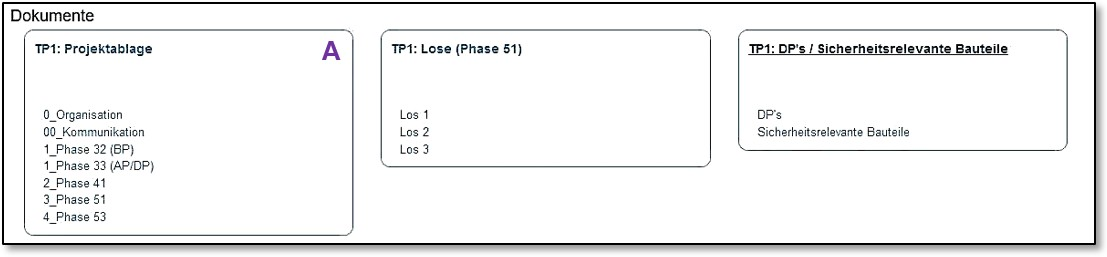
\includegraphics[width=1\linewidth]{../chapters/03_RBS/pictures/01_Dok_Overview_cut.jpg}}
% \caption{Neue Sitzung erfassen}
% \label{fig:speciation}
\end{figure}

Sie können wie gewohnt nach den Tags filtern oder via Navigationsbox die Tags suchen und auswählen \col{(A)}.

Im Bearbeitungsmodus (
\includegraphics[height=12pt]{/Icons/bearbeiten.jpg}) wurde die Handhabung mit den Tags in der Version 2.11 überarbeitet und bietet eine übersichtlichere Auswahl der Tags:

\begin{figure}[H]
\center{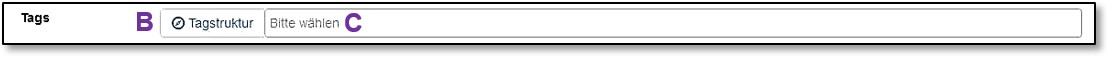
\includegraphics[width=1\linewidth]{../chapters/03_RBS/pictures/02_Dok_Edit_cut.jpg}}
% \caption{Neue Sitzung erfassen}
% \label{fig:speciation}
\end{figure}

Neu finden Sie  den Button 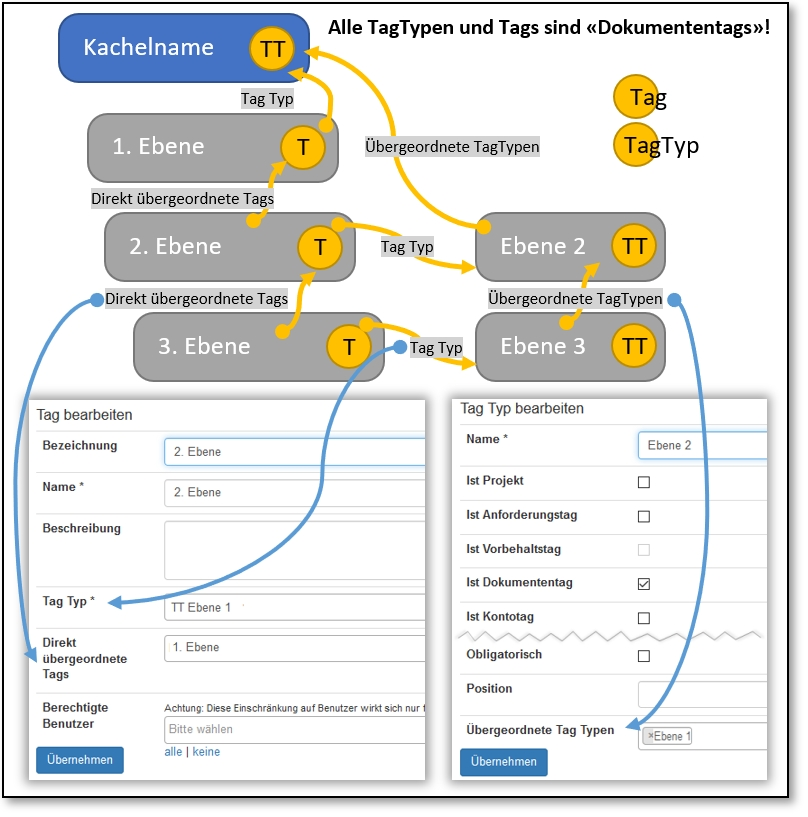
\includegraphics[height=12pt]{/Icons/Tagstruktur.jpg} \col{(B)}, mit welchem Sie direkt die neue Navigation der Tags aufrufen:

% \pagebreak

\begin{wrapfigure}[13]{l}{6.5cm}   % [x] Wie manche Zeile soll sich um die Grafik "brechen"
  \vspace{-23pt}      % Grundwert war 20; mit 30 schön oben beim Text ausgerichtet
  \begin{center}
    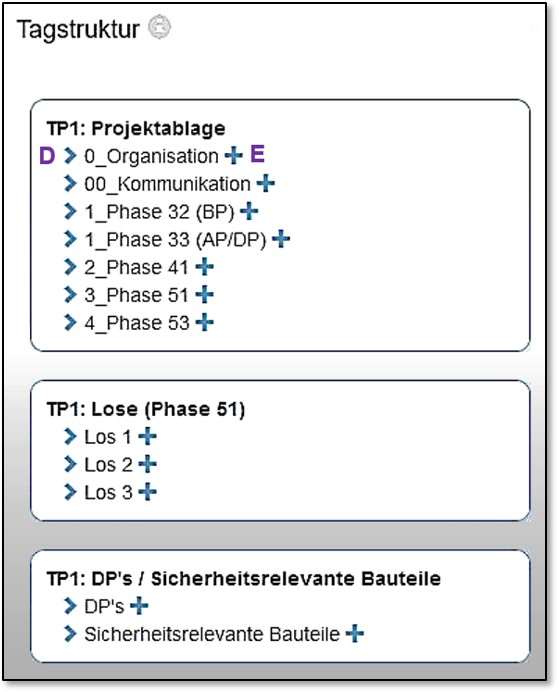
\includegraphics[width=1\linewidth]{../chapters/03_RBS/pictures/04_Dok_Struktur_eingeklappt.jpg}
  \end{center}
  \vspace{-20pt}
%  \caption{Das Menü verwenden}
  \vspace{-10pt}
\end{wrapfigure}

\textbf{Anwendung}: Navigieren Sie mit 
\includegraphics[height=12pt]{/Icons/Pfeil_rechts.jpg} \col{(D)} und klicken Sie hinter dem gesuchten Tag auf das 
\includegraphics[height=12pt]{/Icons/Pluszeichen.jpg}-Zeichen \col{(E)} (Mehrauswahl von Tags ist möglich) und schliessen Sie das Tag-Fenster oben rechts mit 
\includegraphics[height=12pt]{/Icons/X_Button.jpg}. Die Tags wurden im Feld Tags übernommen und können dort auch wieder gelöscht werden.

\vspace{\baselineskip}

\textbf{Hinweis}: Wenn Sie auf der Bearbeitungsseite (
\includegraphics[height=12pt]{/Icons/bearbeiten.jpg}) unter Tags Stichworte eingeben \col{(C)}, wird nach zutreffenden Tags gesucht. Werden diese dort angeklickt, öffnet sich die Tag-Struktur und Sie werden gleich zum ausgewählten Tag geführt. Mit Klick auf das Pluszeichen (
\includegraphics[height=12pt]{/Icons/Pluszeichen.jpg}) wird dieser Tag übernommen. Weitere Tags können angewählt werden. Mit Klick oben rechts im Tag-Fenster (
\includegraphics[height=12pt]{/Icons/X_Button.jpg}) verlassen Sie die Übersicht. Die ausgewählten Tags werden in die Bearbeitungsseite übernommen und können auch wieder gelöscht werden.

\pagebreak
\subsection{Änderungen beim Sitzungswesen:} % Sub-section

\textbf{Globaler Überarbeitungsmodus}:
In der Ansicht 'Protokoll bearbeiten' können Sie den globalen Überarbeitungsmodus ein- und ausschalten. 

\begin{figure}[H]
\center{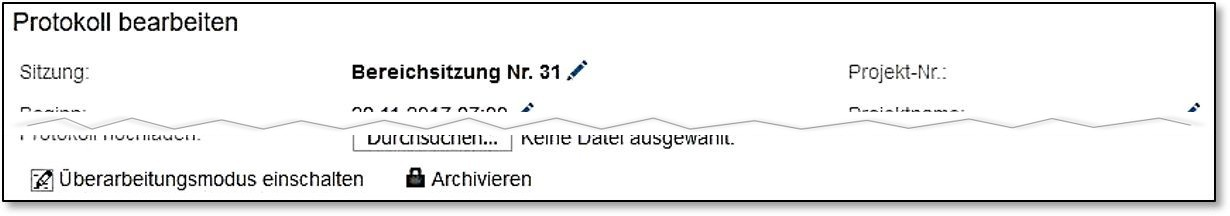
\includegraphics[width=1\linewidth]{../chapters/03_RBS/pictures/SW_SiBearbeiten_cut.jpg}}
% \caption{Neue Sitzung erfassen}
% \label{fig:speciation}
\end{figure}

Mit einem Klick alle Änderungen bei den Traktandeneinträge annehmen oder ablehnen:

\begin{figure}[H]
\center{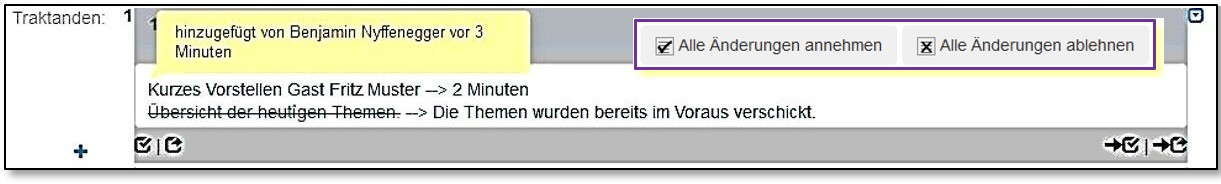
\includegraphics[width=1\linewidth]{../chapters/03_RBS/pictures/SW_Ueberarbeiten_cut.jpg}}
% \caption{Neue Sitzung erfassen}
% \label{fig:speciation}
\end{figure}

\textbf{Offene Pendenzen mit einem Klick abrufbar}:
Bei 'Sitzungseinladung bearbeiten' und 'Protokoll bearbeiten' können Sie mittels dem 
\includegraphics[height=12pt]{/Icons/Fahne.jpg}-Icon mit einem Klick direkt auf die offenen Pendenzen wechseln, welche im Zusammenhang mit der Sitzung stehen:

\begin{figure}[H]
\center{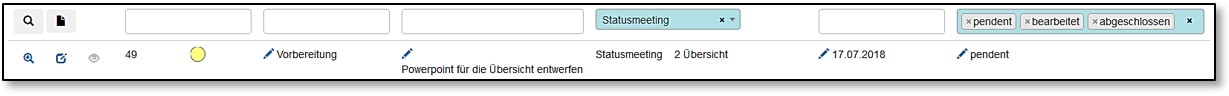
\includegraphics[width=1\linewidth]{../chapters/03_RBS/pictures/Pend_Ueb_cut.jpg}}
% \caption{Neue Sitzung erfassen}
% \label{fig:speciation}
\end{figure}

% \vspace{\baselineskip}
% \pagebreak

\textbf{Anhänge bei der Termineinladung und beim Protokoll-Versand}:

Dateien, welche Sie per Link 
\includegraphics[height=12pt]{/Icons/Link.jpg} oder mittels Hochladen 
\includegraphics[height=12pt]{/Icons/Pluszeichen.jpg} an eine Termineinladung oder einem Protokoll angehängt haben, werden bei der Einladung oder beim Protokoll-Versand als Attachment angehängt:

\begin{figure}[H]
\center{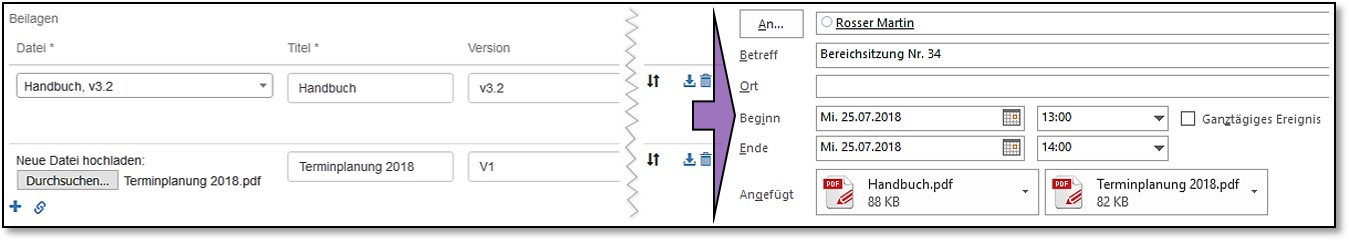
\includegraphics[width=1\linewidth]{../chapters/03_RBS/pictures/Anlagen.jpg}}
% \caption{Neue Sitzung erfassen}
% \label{fig:speciation}
\end{figure}

\textbf{Protokollversand}: Sitzungsteilnehmer mit Status 'Eingeladen' stehen im Mailprogramm unter 'An', mit Statuts 'Verteiler' unter 'Cc':

\begin{figure}[H]
\center{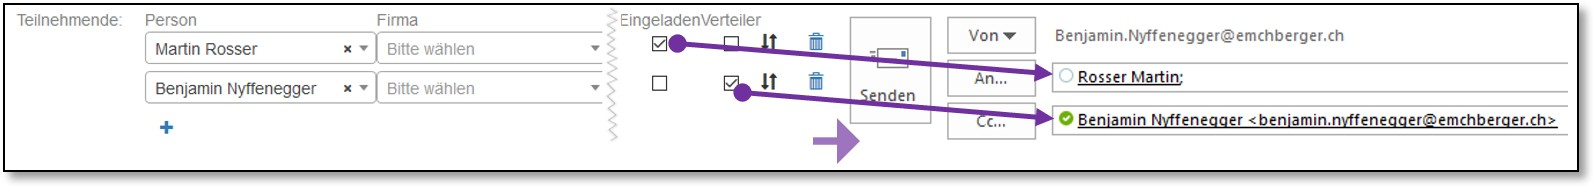
\includegraphics[width=1\linewidth]{../chapters/03_RBS/pictures/Versand.jpg}}
% \caption{Neue Sitzung erfassen}
% \label{fig:speciation}
\end{figure}
		
\subsection{Weiterführende Informationen und Support} % Sub-section

Die Detailbeschreibung finden Sie im CUBE PA-Benutzerhandbuch. Für weitere Fragen kontaktieren Sie uns unter {\color{red} cube.support@emchberger.ch}.
